\documentclass[onecolumn, draftclsnofoot, 10pt, compsoc]{IEEEtran}
\usepackage{graphicx}
\graphicspath{{./figures/}}

\usepackage{url}
\usepackage{setspace}
\usepackage{multicol}
\usepackage{pdflscape}
\usepackage{pdfpages}
\usepackage[british]{babel}
\usepackage{listings}
\usepackage{xcolor}
\usepackage{listings}
\usepackage{hyperref}
\usepackage{subfig}
\usepackage{pdfpages}
\usepackage{longtable}

\usepackage{geometry}
\geometry{textheight=9.5in, textwidth=7in}

\hypersetup{
    colorlinks=true,
    linkcolor=blue,
    filecolor=magenta,      
    urlcolor=cyan,
}

% \overfullrule=2in

% 1. Fill in these details
\def \CapstoneTeamName{			Ground Station Software Team}
\def \CapstoneTeamNumber{		30}
\def \GroupMemberOne{			Kenneth Steinfeldt}
\def \GroupMemberTwo{			Christopher Pham}
\def \GroupMemberThree{			Corwin Perren}
\def \CapstoneProjectName{		OSU Robotics Club\\Mars Rover Ground Station}
\def \CapstoneSponsorCompany{	OSU Robotics Club}
\def \CapstoneSponsorPerson{	Nick McComb}



%Personal \newcommands

\newcommand{\functRequ}[4]{
\item #1%
\par
\begin{itemize}
\item \textit{Description:} #2.%
\item \textit{Rationale:} #3.%
\item \textit{Dependencies:} #4%
\end{itemize}
}
\definecolor{backcolor}{rgb}{0.95,0.95,0.92}
\lstset{basicstyle=\ttfamily,
  backgroundcolor=\color{backcolor},  
  showstringspaces=false,
  commentstyle=\color{red},
  keywordstyle=\color{blue},
  columns=fullflexible,
  breaklines=true,
  postbreak=\mbox{\textcolor{red}{$\hookrightarrow$}\space},
}


% 2. Uncomment the appropriate line below so that the document type works
\def \DocType{	%Problem Statement
				%Requirements Document
				%Technology Review
				%Design Document
				Final Report
			 }
			
\newcommand{\NameSigPair}[1]{
  \par
  \makebox[2.75in][r]{#1} 
  \hfill
  \makebox[3.25in]{
      \makebox[2.25in]{\hrulefill} 
      \hfill
      \makebox[.75in]{\hrulefill}
  }
  \par\vspace{-12pt} 
  \textit{
      \tiny\noindent
      \makebox[2.75in]{} 
      \hfill
      \makebox[3.25in]{
          \makebox[2.25in][r]{Signature} 
          \hfill
          \makebox[.75in][r]{Date}
      }
  }
}
% 3. If the document is not to be signed, uncomment the command below
\renewcommand{\NameSigPair}[1]{#1}

%%%%%%%%%%%%%%%%%%%%%%%%%%%%%%%%%%%%%%%
\begin{document}
\begin{titlepage}
	\pagenumbering{gobble}
	\begin{singlespace}
		% 4. If you have a logo, use this includegraphics command to put it on the coversheet.
        \begin{minipage}{7in}
			\centering
			\hspace*{-.7in}
			$\vcenter{\hbox{
\includegraphics[height=4cm]{Oregon_State_College_of_Engineering_Logo}}}$
			\hspace*{.2in}
			$\vcenter{\hbox{
\includegraphics[height=2.5cm]{OSURCLogoOrange}}}$
		\end{minipage}

		\par\vspace{.35in}
		\centering
		\scshape{
			\huge CS Capstone \DocType \par
			{\large\today}\par
			\vspace{.5in}
			\textbf{\Huge\CapstoneProjectName}\par
			\vfill
			{\large Prepared for}\par
			\Huge \CapstoneSponsorCompany\par
			\vspace{5pt}
			{\Large\NameSigPair{\CapstoneSponsorPerson}\par}
			{\large Prepared by }\par
			Group\CapstoneTeamNumber\par
			% 5. comment out the line below this one if you do not wish to name your team
			\CapstoneTeamName\par 
			\vspace{5pt}
			{\Large
				\NameSigPair{\GroupMemberOne}\par
				\NameSigPair{\GroupMemberTwo}\par
				\NameSigPair{\GroupMemberThree}\par
			}
			\vspace{20pt}
            \begin{abstract}
			% 6. Fill in your abstract
			This document contains all of the useful documentation about the OSURC Mars Rover ground station project as it has progressed throughout the year. This includes all technical documents (with revisions), weekly blog posts, code documentation, and lessons learned.

		\end{abstract}
		}
	\end{singlespace}
\end{titlepage}
\newpage
\pagenumbering{arabic}
\tableofcontents
\clearpage

% Write stuff here....
\section{Introduction}
\subsection{Who Requested the Project?}
This project was requested by the Oregon State University Robotics Club's (OSURC) Mars Rover team.

\subsection{Why Was the Project Requested?}
This project was requested due to the Mars Rover team's need for a complete and functional ground station in a time frame that the existing software team may not have been able to accomplish. Additionally, new requirements for the ground station meant that the increased complexity was most likely going to require a more dedicated team to complete than the volunteers the club normally has working on the Mars Rover project.

\subsection{What is the Importance of the Project?}
This project solves some of the most common problems for the Mars Rover team in previous competition years. Historically, the team is allowed a 10-15 minute set up time during competition where the Rover must be turned on, ground station connected, and core systems tested before actually competing in a task. In previous years, the Rover's ground station has normally been a laptop with a handful of random pieces of hardware plugged into it over USB. Many times, this hardware has been damaged during transit and caused problems during the setup phase. Additionally, previous software has often been command line driven and extremely specialized meaning the software is difficult to use, difficult to teach, and has ended up getting re-written with each new Rover competition year.

\subsection{Our Client and Their Role}
Our client was Nick McComb, team lead and electrical lead of the Mars Rover team for the 2017-2018 competition year. His role was mainly supervisory, helping our group set up the initial requirements for the software, and occasionally making requests for additional features as the year progressed. 

\subsection{Our Team Members and Roles}
\begin{itemize}
\item Chris Pham
	\begin{itemize}
    \item Rover mapping systems
	\end{itemize}
\item Ken Steinfeldt
	\begin{itemize}
    \item Rover status systems
	\end{itemize}
\item Corwin Perren
	\begin{itemize}
	\item Team Manager
    \item Rover video systems
    \item Program structure / startup
	\end{itemize}
\end{itemize}

\section{Requirements Document}
\subsection{Original Document}
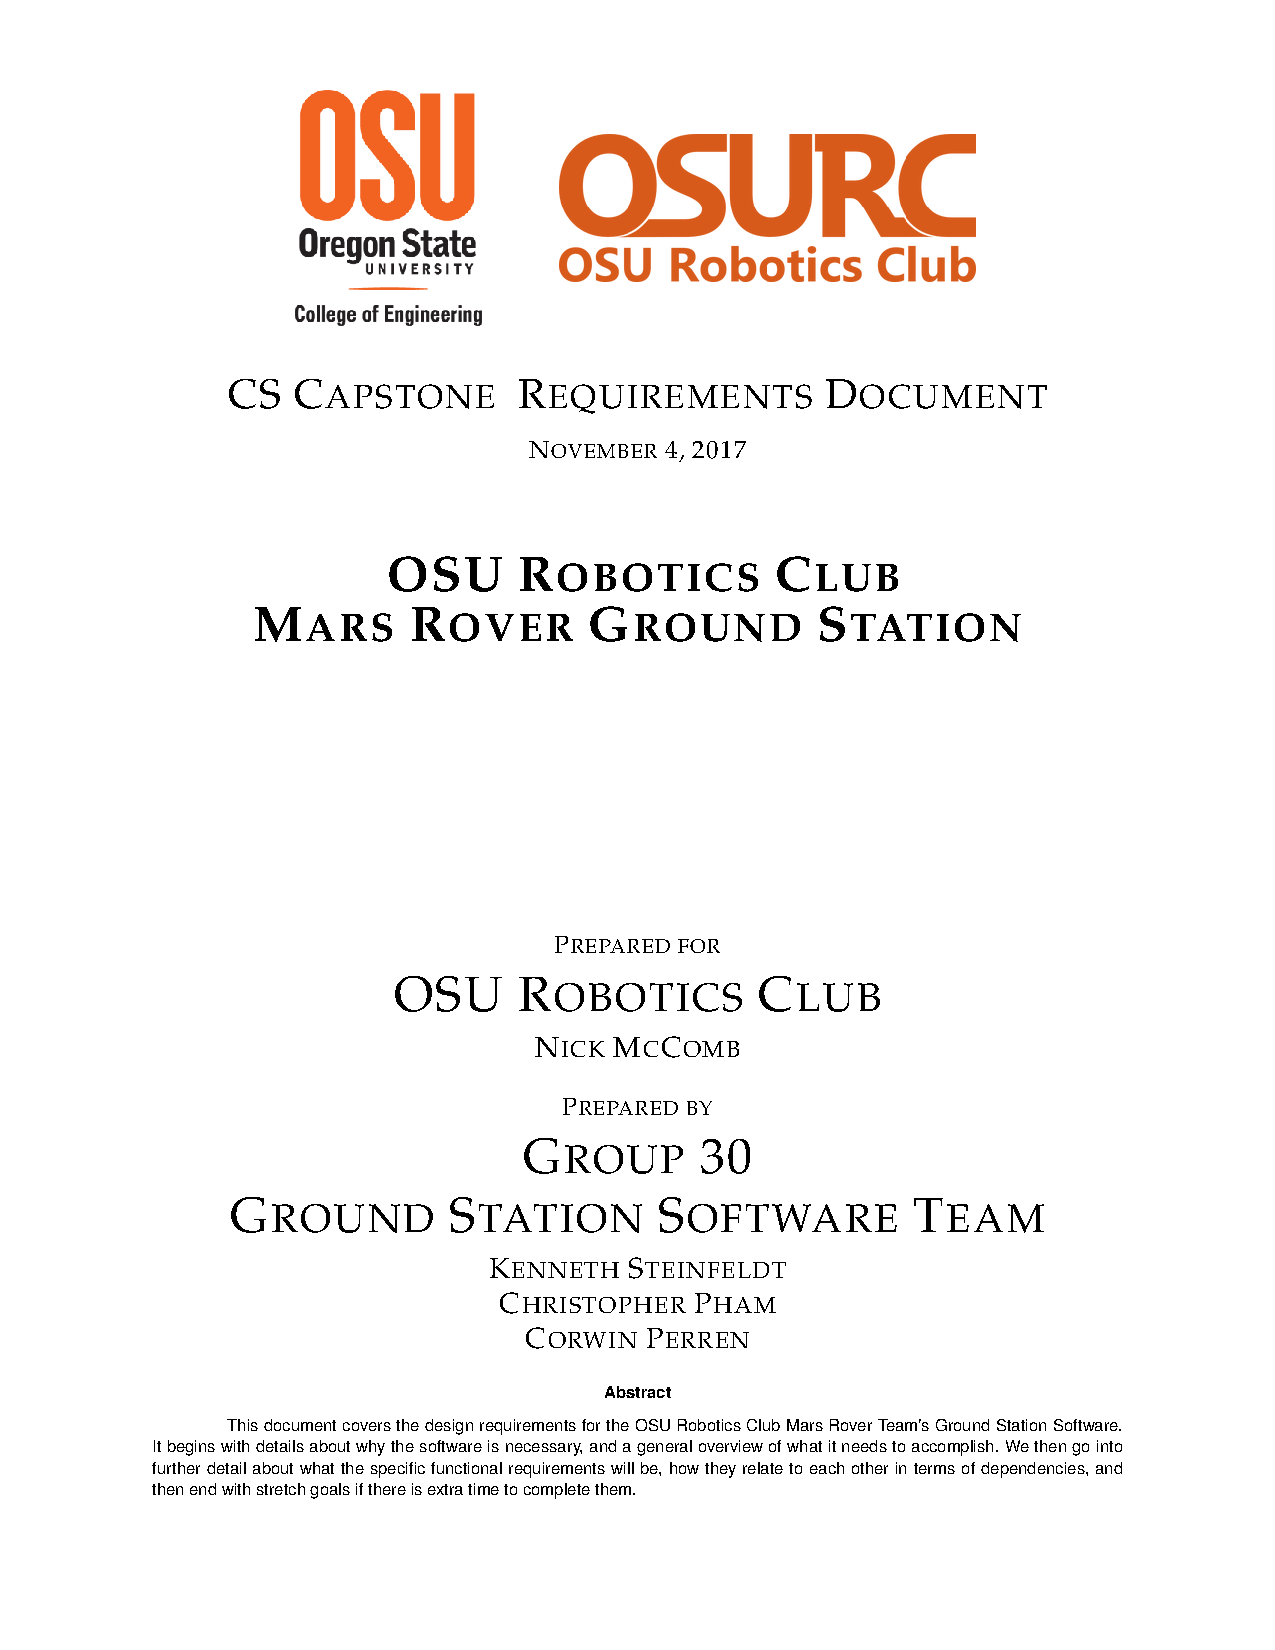
\includepdf[pages=-, frame=true, scale=0.95]{02-requirementsdoc/group-design-requirements.pdf}

\subsection{Additions}
\subsubsection{Final Revision Document}
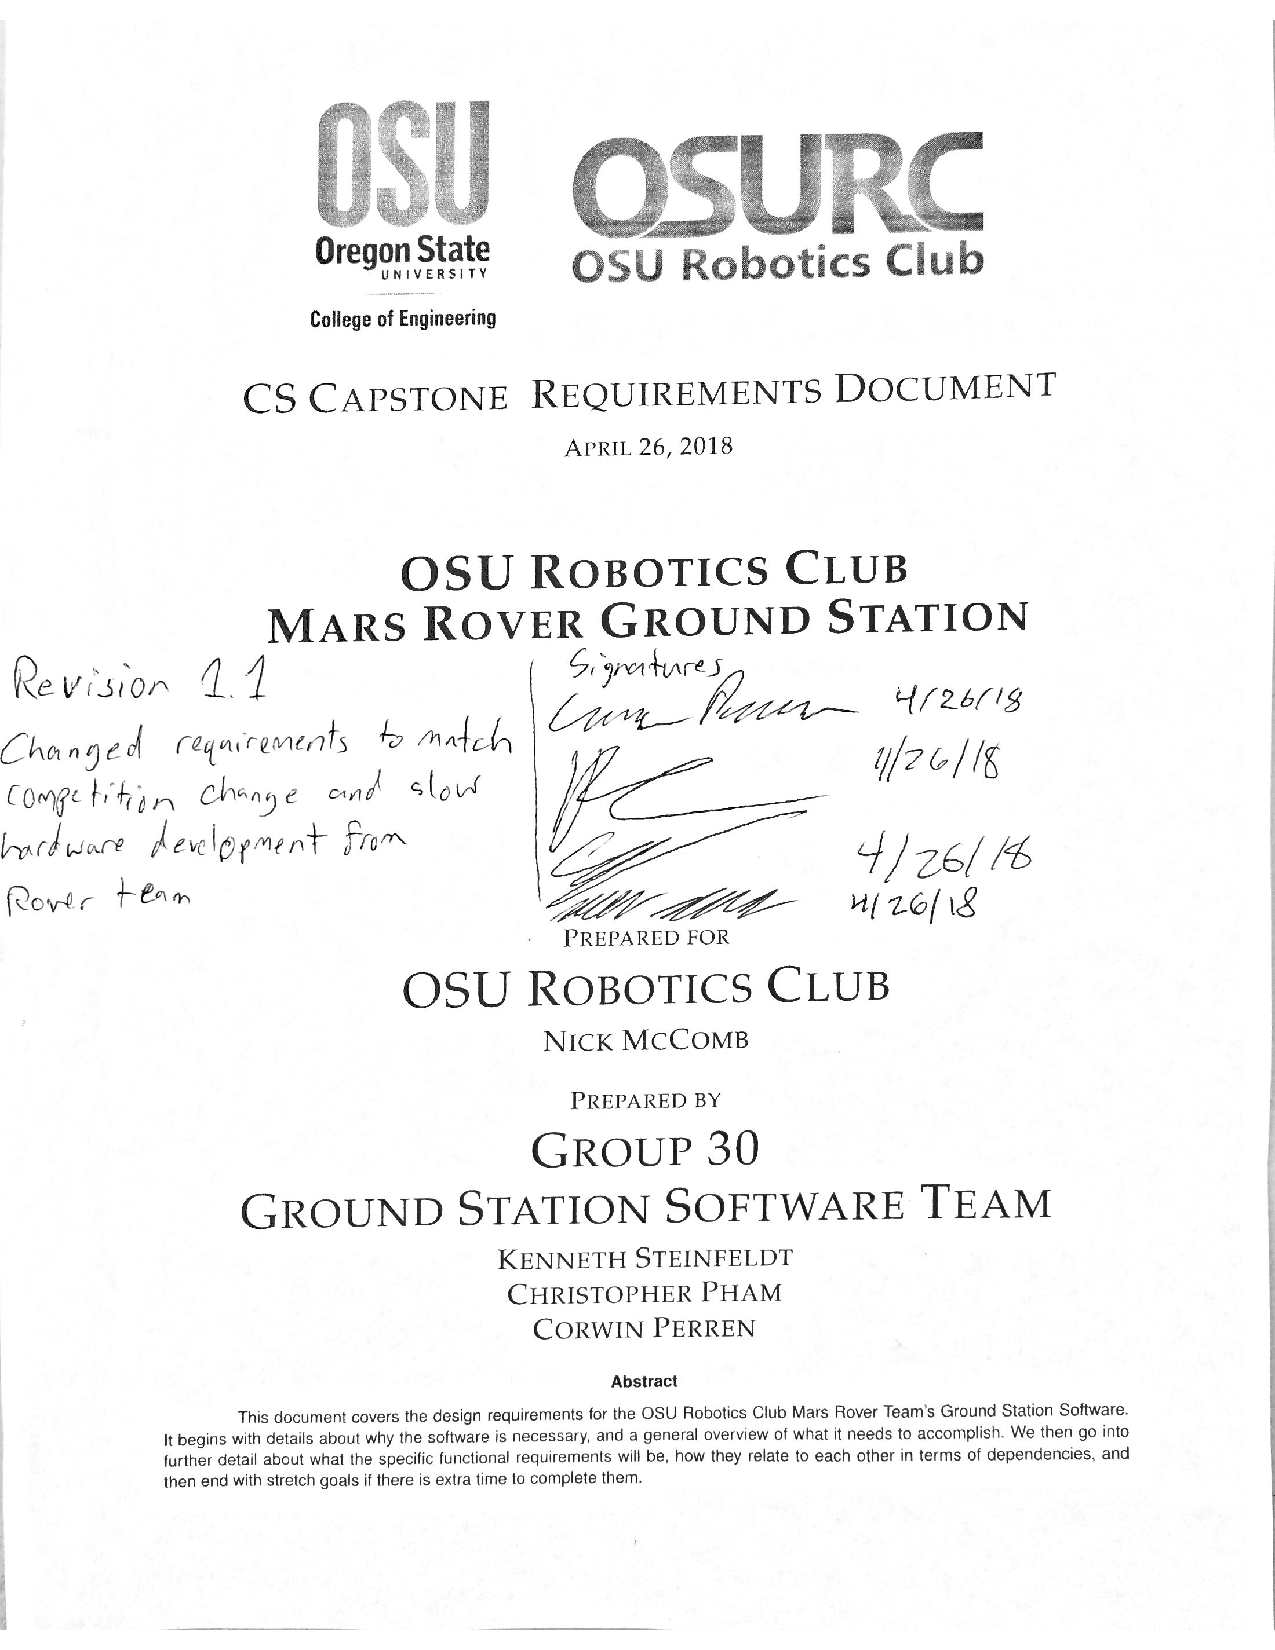
\includepdf[pages=-, frame=true, scale=0.95]{02-requirementsdoc/cs_group30_design_requirements_revision1_1.pdf}

\subsubsection{Description of Changes}
Version 1.1 of document was approved by all team members and stakeholder on 4/26/2018.

\begin{itemize}
\item Edited descriptions of competition from University Rover Challenge to Canadian International Rover Challenge
	\begin{itemize}
	\item The Mars Rover team changed competitions, so we updated the document to reflect this
	\end{itemize}
    
\item Removed user story for manual video quality adjustment
	\begin{itemize}
	\item Our team implemented automatic quality adjustment, so manual adjustment was no longer necessary
	\end{itemize}
    
\item Removed user story about easily seeing when an autonomous run has completed
	\begin{itemize}
	\item The new Rover competition does not require this display element
	\end{itemize}
    
\item Removed user story about needing to view live logs
	\begin{itemize}
	\item Log viewing was determined to not be needed as there would be too many logs to sort through in a short amount of time
	\end{itemize}
    
\item Removed user story about seeing network latency (round trip time)
	\begin{itemize}
	\item The network connection percentage was determined to be correlated with this value enough that this redundant element was not needed
	\end{itemize}

\item Added constraint that the GUI software must have placeholder for GUI elements and software features that can not be completed due to waiting on Rover team progress
	\begin{itemize}
	\item Our team encountered many situations where we could not continue development due to lack of hardware/software on Rover
    \item This new constraint allows us to still meet requirements if the bottleneck is the Rover team
	\end{itemize}
    
\item Changed functional requirement for joystick statuses so that the SpaceNav mouse had its own requirement
	\begin{itemize}
	\item The team changed to a SpaceNav mouse earlier in the year and it was determined that an individual readout for this input device would be convenient
	\end{itemize}
    
\item Changed functional requirement for battery status to battery voltage
	\begin{itemize}
	\item The battery status value was determined to be most useful as a voltage, rather than a percentage estimate
	\end{itemize}
    
\item Removed functional requirement for Rover voltage statuses
	\begin{itemize}
	\item The Rover design changed so that only the battery voltage is measured
	\end{itemize}
    
\item Changed functional requirement for bogie connection statuses to be individual wheel statuses
	\begin{itemize}
	\item The Rover software team got individual status information for each wheel, rather than a two wheel bogie group, and requested this change
	\end{itemize}
    
\item Removed functional requirement for Rover network round trip time
	\begin{itemize}
	\item The network connection percentage was determined to be correlated with this value enough that this redundant element was not needed
	\end{itemize}
    
\item Changed functional requirement for Rover arm joystick control to SpaceNav mouse control
	\begin{itemize}
	\item The team changed to a SpaceNav mouse over a second joystick for arm control
	\end{itemize}
    
\item Removed functional requirement for way-point navigation path
	\begin{itemize}
	\item Expectations for how autonomy on the Rover would work would not easily give our team this information to display
	\end{itemize}
    
\item Changed functional requirement for the autonomy indicator so that it shows whether autonomy is active rather than when autonomy is finished
	\begin{itemize}
	\item Changing to the Canadian International Rover Challenge made the old requirement unnecessary
	\end{itemize}
    
\item Removed functional requirement for video FPS counters
	\begin{itemize}
	\item FPS counters would have been useful for manual video quality adjustment, but are no longer needed with automatic quality adjustment
	\end{itemize}
    
\item Removed functional requirement for log file viewing
	\begin{itemize}
	\item Log files were too large to usefully sort through in a short amount of time
	\end{itemize}
    
\end{itemize}

\subsection{Final Gantt Chart}
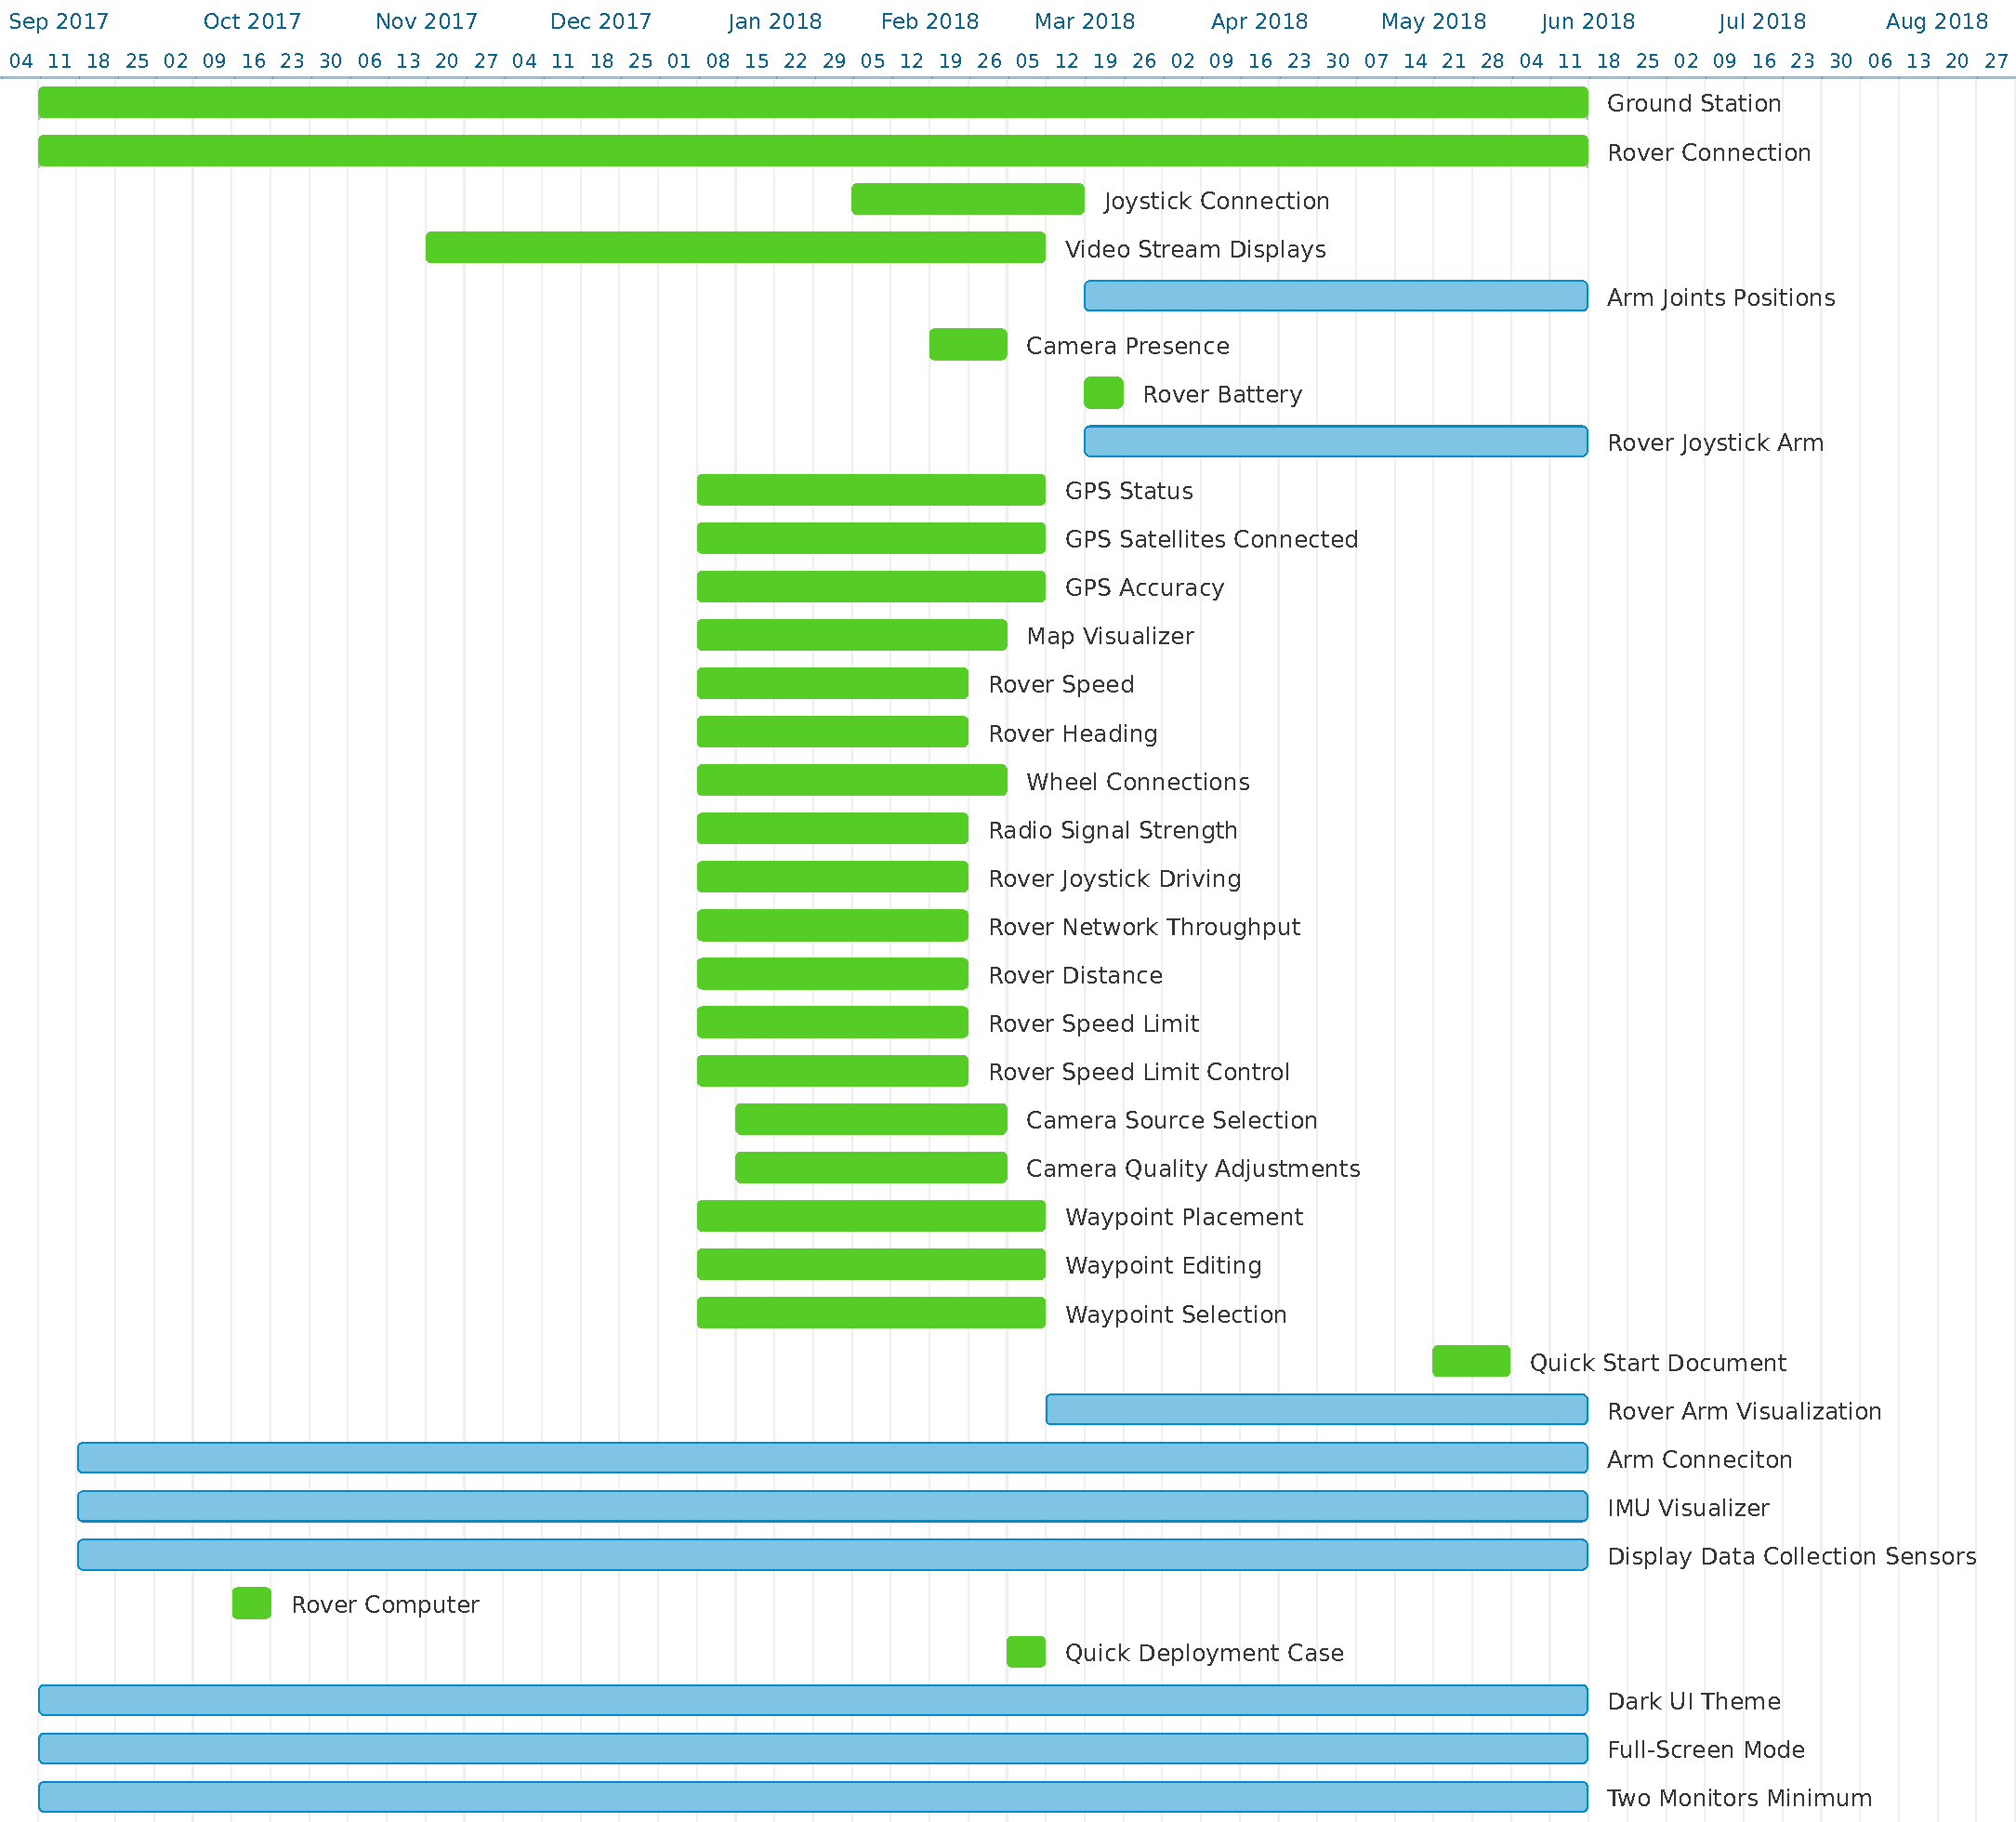
\includepdf[pages=-, frame=true, landscape, scale=0.95]{02-requirementsdoc/final_gantt.pdf}
\section{Design Document}
\subsection{Original Document}
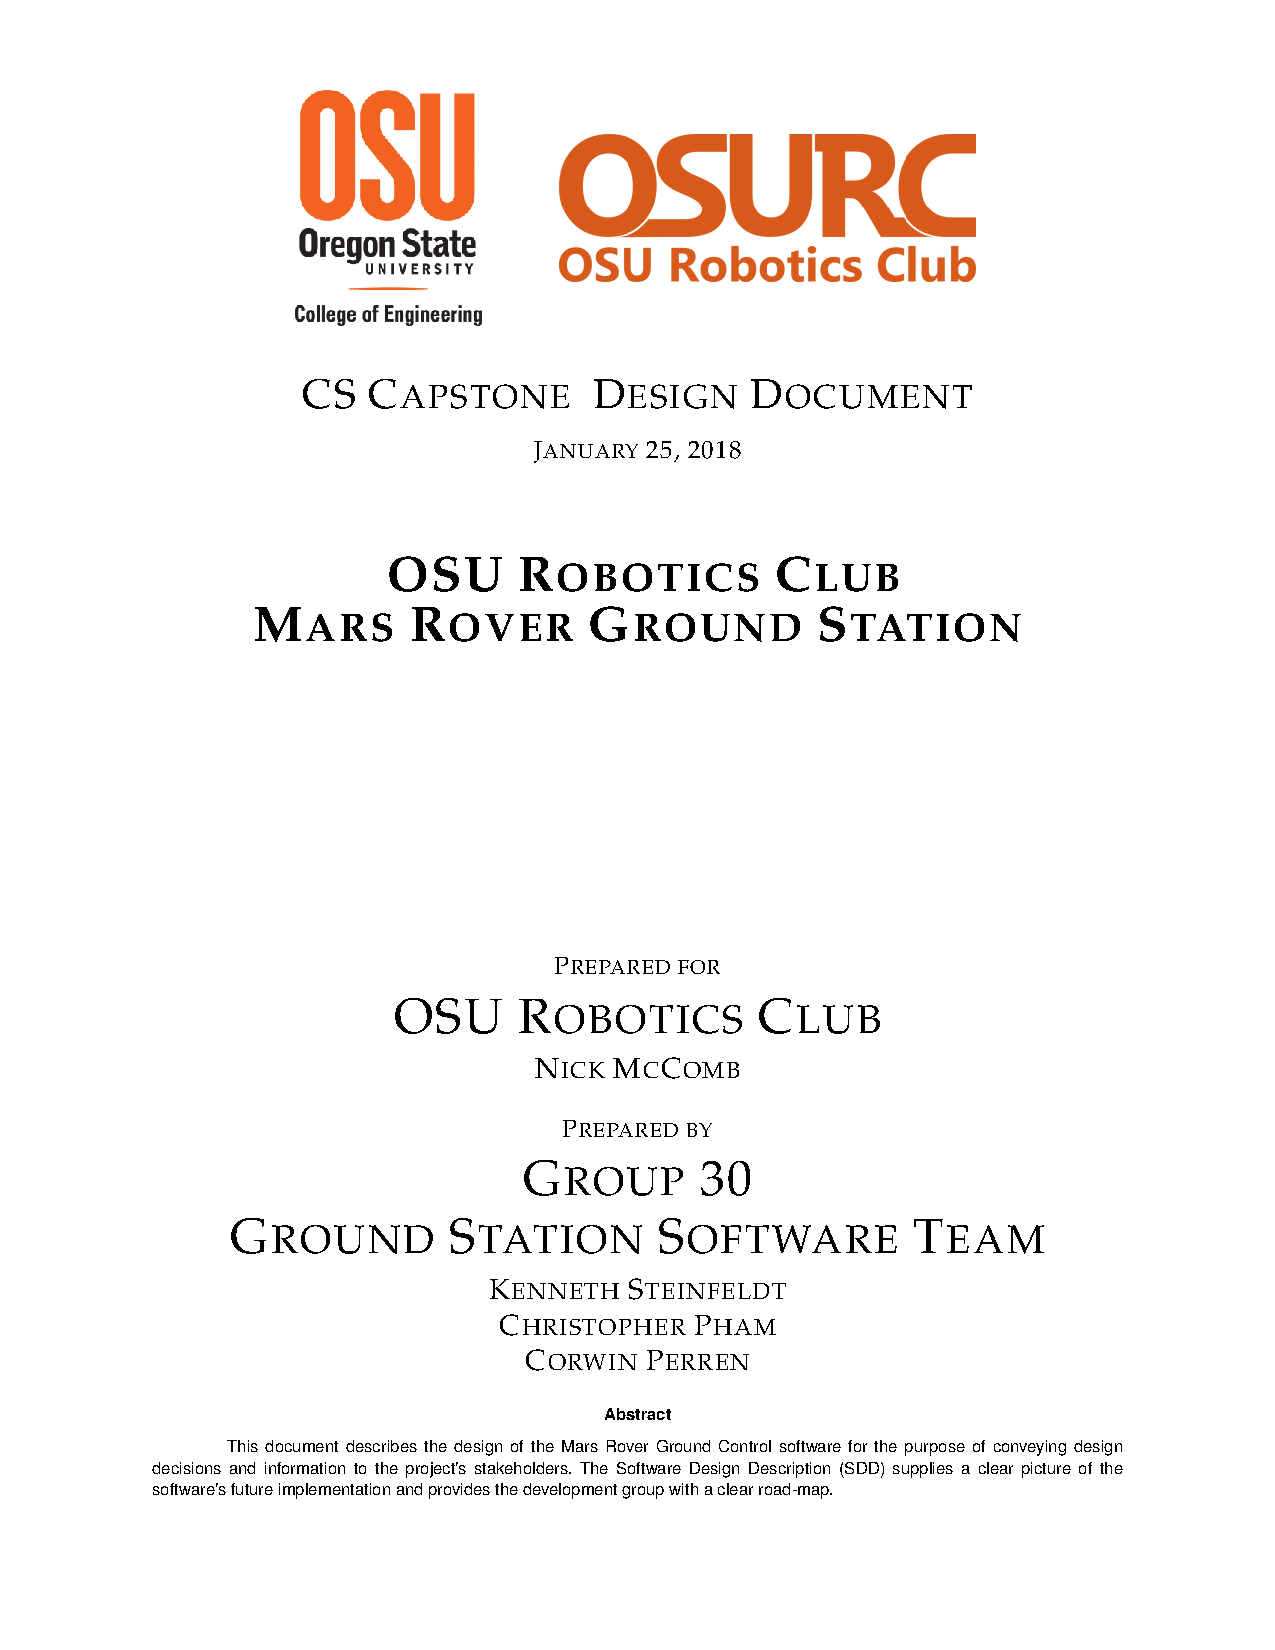
\includepdf[pages=-, frame=true, scale=0.95]{03-designdoc/group-design-document.pdf}
\subsection{Additions}
There were no additions to our original design document.
\section{Tech Review Document}
\subsection{Original Documents}
\subsection{Chris Pham}
\subsubsection{Week 1}
During the start of the term, I personally did not work on much because of issues with registration 
However, we did work out when we are expecting to work and meet up this term, which would be on Thursdays around 10 o'clock in the morning.
\subsubsection{Week 2}
This week, I worked on completing the integration of the GUI.
It turned out last term, that the East/West portion of the DMS conversion was not being set correctly.
I spent a bit of time trying to get the correct float value to go down but then my minutes was completely off to the calculated DMS of the GPS location.
Turns out that the box that contained the DMS location, would be limited to 0, 90, which actually needs to be 180 because it needs to span a half circle.
Once that value was changed, the values were being set correctly.
\subsubsection{Week 3}
Turns out that I forgot to set the sign of the longitude and latitude to their corresponding North/South and East/West values.
That was easily done using with many possible implementations like equalities, sign function in python, and other things like that.
\subsubsection{Week 4}
This week we worked on fixing our poster and fixing our documentation to fit the new specification that the new competition is now the CIRC (Canadian International Rover Challenge) instead of URC.
\subsubsection{Week 5}
During Week 5, I worked on two important things, multi-threading the downloading of the image files from Google and integration of inputs into my mapping system.

\noindent Multi-threading was done using and starting a list of processes that have access to a download function in the class.
I could not of done a pool because of the issues I was getting like the pickling issues in Python in trying to pack the state.
Another issue that came with this implementation, was the rate limitations that the server was sending.
To combat both issues, I implemented a bounded semaphore instead a normal semaphore, because a bounded version of it will return an error whenever the process tries to obtain a lock.
One big issue is still combining the files because that is still done in square time.
One optimization should be splitting work into its smallest parts and then combining them, however, trying to merge all the files correctly ended up being the biggest issue I had.

\noindent Also have started on integrating the GPS data that we are getting and applying that onto the map system that I've created.
One problem is I forget how the data is formatted in the system and I need direct access to view the data that is being sent by the rover to parse correctly.
\subsubsection{Ken Steinfeldt}

\includepdf[pages=-, frame=true, scale=0.95]{04-techreviewdocs/steinfek-tech-report.pdf}
\subsubsection{Corwin Perren}

\includepdf[pages=-, frame=true, scale=0.95]{04-techreviewdocs/tech_review_perrenc.pdf}

\section{Individual Blog Posts}
\subsection{Chris Pham}
\subsubsection{Week 1}
During the start of the term, I personally did not work on much because of issues with registration 
However, we did work out when we are expecting to work and meet up this term, which would be on Thursdays around 10 o'clock in the morning.
\subsubsection{Week 2}
This week, I worked on completing the integration of the GUI.
It turned out last term, that the East/West portion of the DMS conversion was not being set correctly.
I spent a bit of time trying to get the correct float value to go down but then my minutes was completely off to the calculated DMS of the GPS location.
Turns out that the box that contained the DMS location, would be limited to 0, 90, which actually needs to be 180 because it needs to span a half circle.
Once that value was changed, the values were being set correctly.
\subsubsection{Week 3}
Turns out that I forgot to set the sign of the longitude and latitude to their corresponding North/South and East/West values.
That was easily done using with many possible implementations like equalities, sign function in python, and other things like that.
\subsubsection{Week 4}
This week we worked on fixing our poster and fixing our documentation to fit the new specification that the new competition is now the CIRC (Canadian International Rover Challenge) instead of URC.
\subsubsection{Week 5}
During Week 5, I worked on two important things, multi-threading the downloading of the image files from Google and integration of inputs into my mapping system.

\noindent Multi-threading was done using and starting a list of processes that have access to a download function in the class.
I could not of done a pool because of the issues I was getting like the pickling issues in Python in trying to pack the state.
Another issue that came with this implementation, was the rate limitations that the server was sending.
To combat both issues, I implemented a bounded semaphore instead a normal semaphore, because a bounded version of it will return an error whenever the process tries to obtain a lock.
One big issue is still combining the files because that is still done in square time.
One optimization should be splitting work into its smallest parts and then combining them, however, trying to merge all the files correctly ended up being the biggest issue I had.

\noindent Also have started on integrating the GPS data that we are getting and applying that onto the map system that I've created.
One problem is I forget how the data is formatted in the system and I need direct access to view the data that is being sent by the rover to parse correctly.
\subsubsection{Ken Steinfeldt}

\includepdf[pages=-, frame=true, scale=0.95]{04-techreviewdocs/steinfek-tech-report.pdf}
\subsubsection{Corwin Perren}

\includepdf[pages=-, frame=true, scale=0.95]{04-techreviewdocs/tech_review_perrenc.pdf}
\section{Poster}
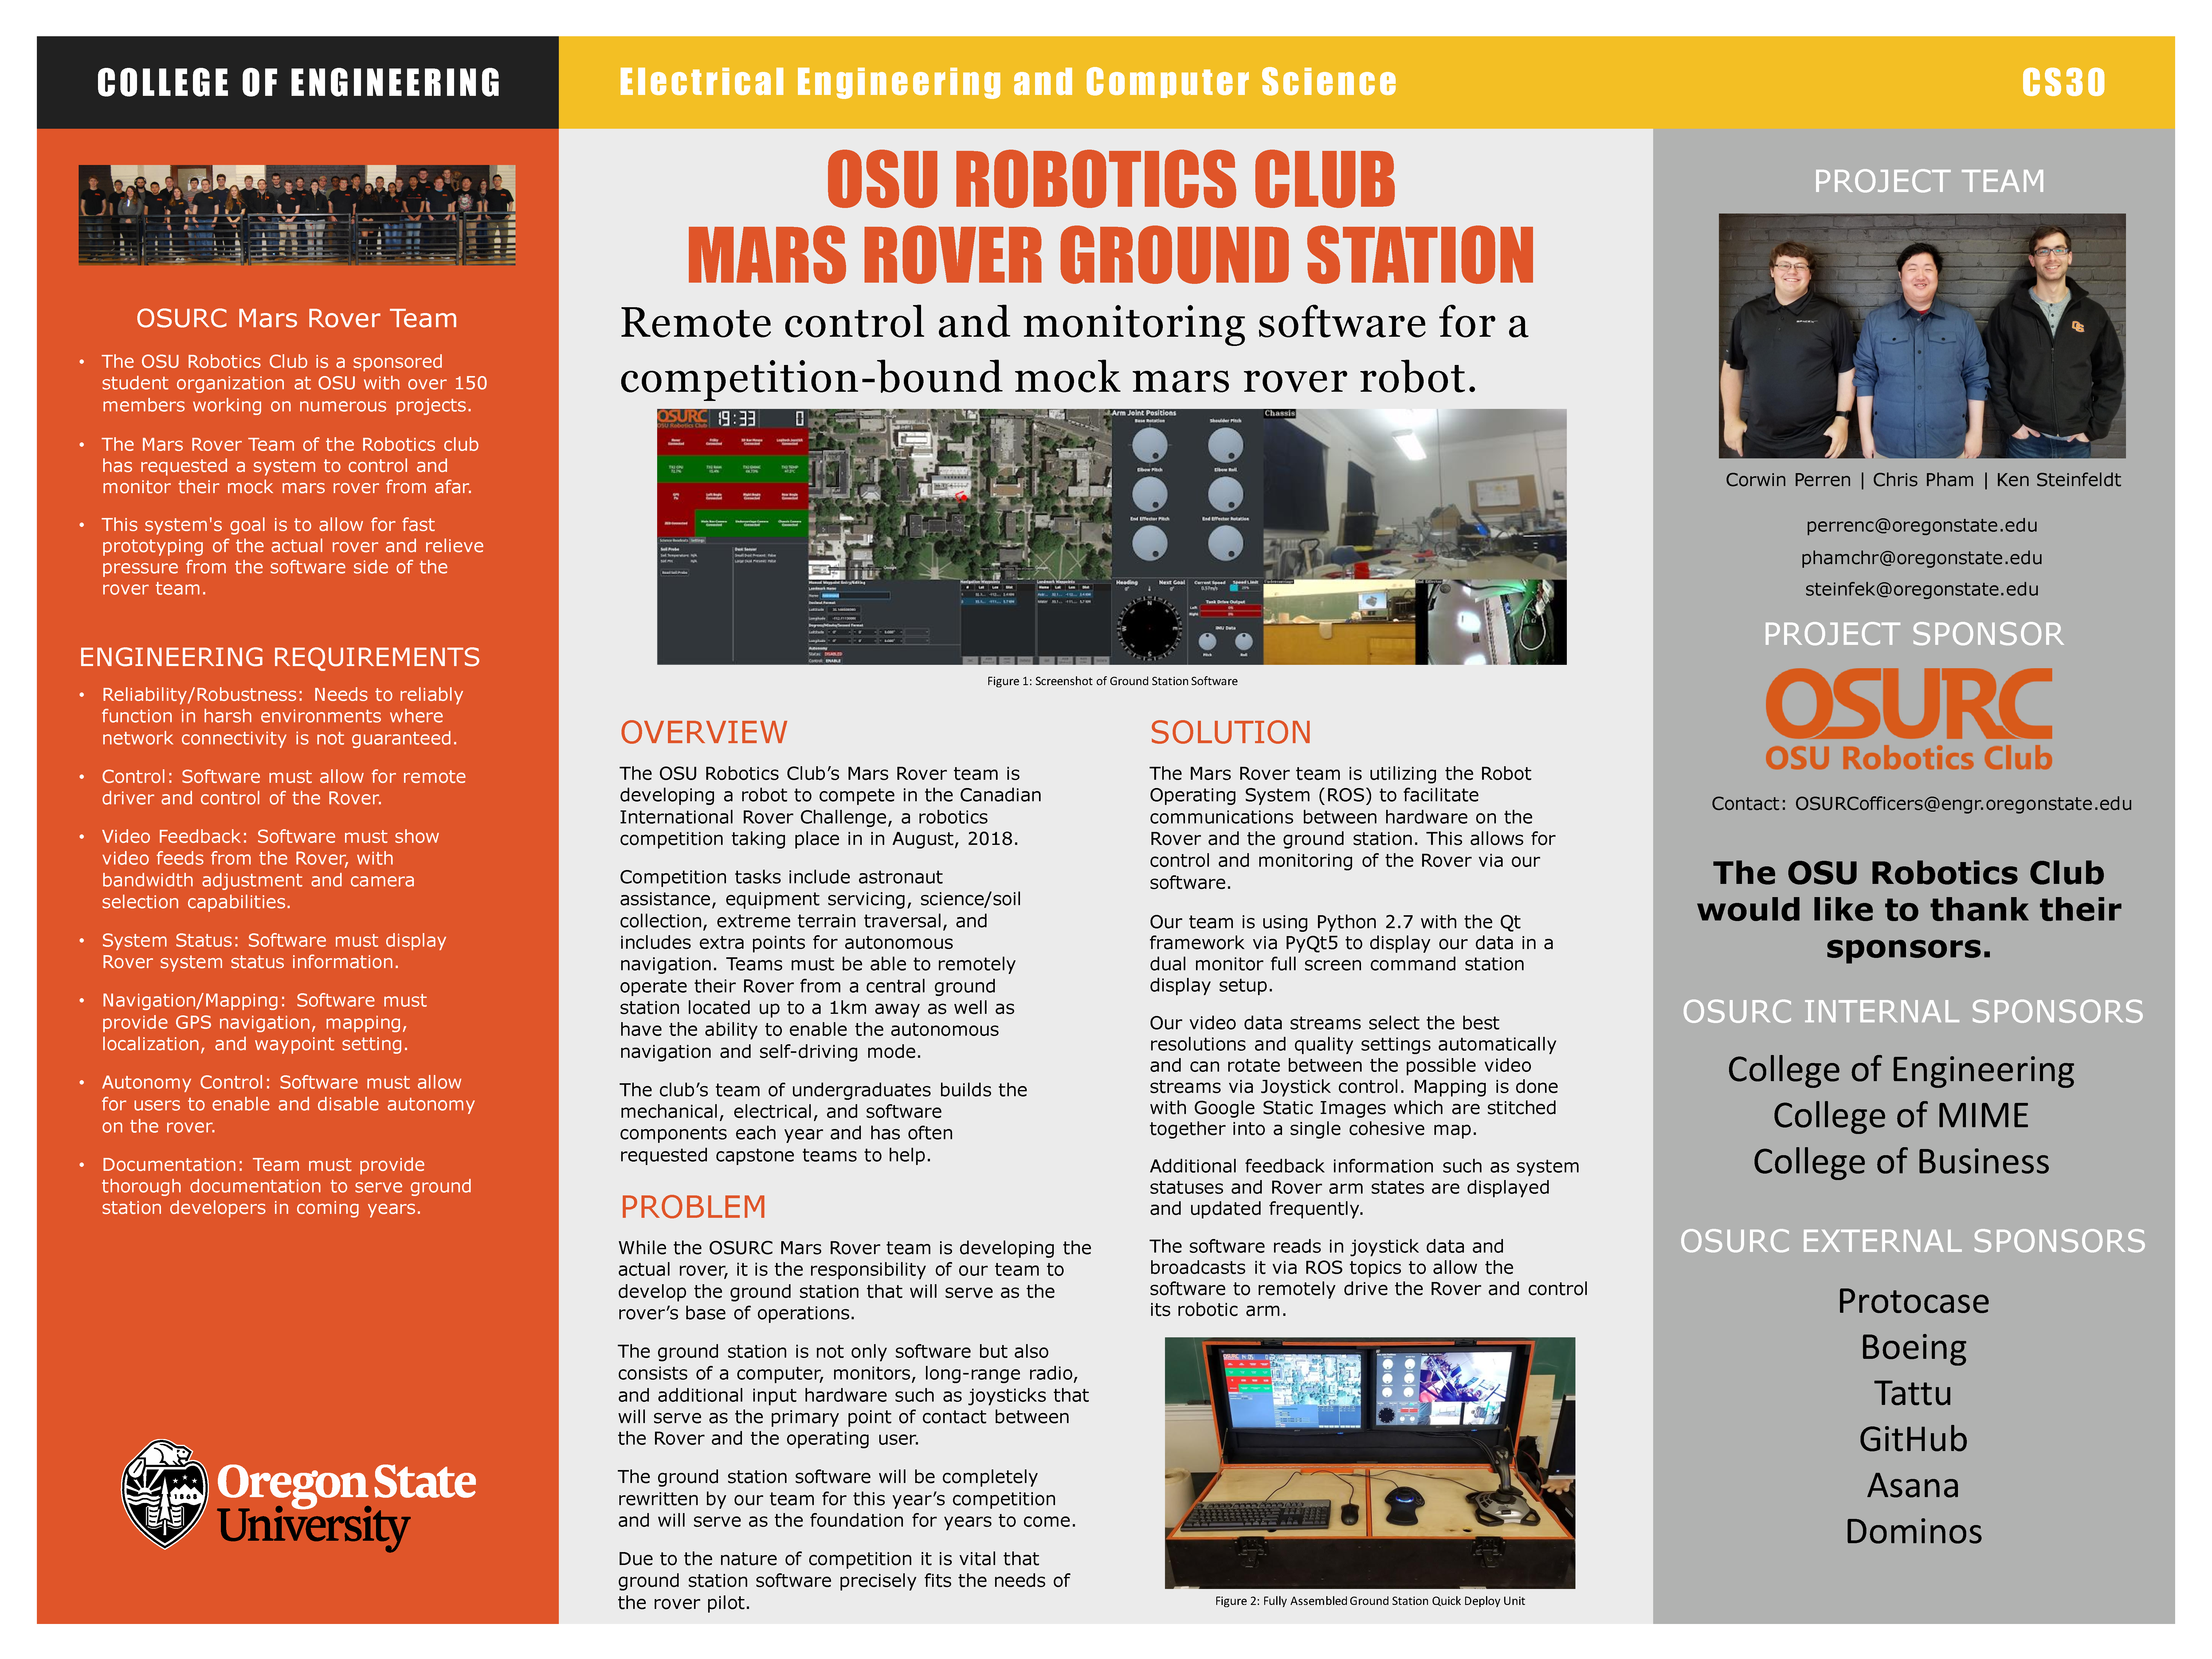
\includepdf[pages=-, scale=1.04, landscape]{06-poster/poster_undergrad_expo_48x36_eecs.pdf}
\section{Documentation}
\subsection{How the Project Works}
\subsubsection{Overview}
This project works by combining the power of Robot Operating System (ROS), the Qt framework, and Python to make a simple (for what it is), fast, easy to modify, and easier to understand piece of software to act as the front end for the Mars Rover. PyQt is used to load and show the UI and give the software programmatic access to GUI elements. It also provides intelligent multi-threading with easy to use cross-thread communication pipelines. The use of python has allowed our team to write this code in a fraction of the time it would have taken in another language such as C++. ROS is the framework that the Rover is running and is based around the concept of abstracting everything into ROS topics. These topics allow for easy sending and receiving of control and status information in a way that is standardized instead of having to use a custom network control protocol.

\subsubsection{Low bandwidth communications}
As the Rover is going to be at long range at many times, having as small of communication packets as possible is a priority. This helps keep control, video, and status information smooth and consistent. In order to facilitate this, the ground station and Rover both are using a package called nimbro\_network that allows for compression of ROS topics and also allows for us to choose between a TCP and UDP transport layer. Non-critical data that we want fast gets sent with compression over UDP and includes video data from the Rover and live drive commands from the ground station. Important and/or infrequent data is sent with or without compression depending and using the TCP transport. Data sent using TCP includes status information from the Rover and, in the future, waypoints and autonomy control. 

\subsubsection{Program Logical Structuring}
To make the ground station software easier to modify and understand, it has been broken down into logical hierarchies. At the core of the ground station source folder are the Framework and Resources folders. The Resources folder contains all of the static assets for the application such as image files and the UI files that determine how the GUI visually looks. The Framework folder contains all of the logical sub-systems of the software such as VideoSystems, InputSystems, and MappingSystems. By separating all systems out like this, it makes it easy to know which files need to be looked at when fixing or adding to the ground station. At the root of the source folder is "ground\_station.py", the launcher file for the whole application. Under normal conditions, this file only needs to be modified if a new threaded class is being added for additional functionality. This file handles launching of the software, displaying the GUI, and management of the startup and shutdown of all running threads.

\subsubsection{Threading \& Adding Classes}
As this is a very large program with many systems running concurrently it has required the use of many threaded classes. To abstract away many of the complexities of this, the ground station main launcher file contains a method called add\_thread used to spin up a new threaded class from the Framework folder when one is made. This method also handles the graceful shutdown of the software when quit. In order for graceful shutdown, all of the program's child threads must not be running when the main launcher thread exits. If this is not the case, the application may hang or maintain unwanted connections in the background after it seems like it has exited. Anyone wishing to add new functionality to the GUI in a new file should copy an existing threaded class to use as a baseline.

\subsubsection{ROS in Python}
ROS is a large part of why this software has been much easier to write than it could have been. In Python, the ROS subsystem can be accessed by importing rospy and calling rospy.init to tell ROS that we have a new node running. At this point, topics can be subscribed to by giving it the topic path and a the data type of the topic. Conversely, to broadcast a new topic message, a publisher is made by providing the topic path, data type, and queue size. To actually broadcast a message, you create a new instance of the data type, fill it with the desired data, and use the publisher's ".publish()" method to send it. In our software, these topics are used for all communications to and from the Rover. Absolutely no custom communication methods are used to interface between the Rover and ground station. An important note about the ROS messages used are that most of these messages are custom defined. In order for rospy and python to know the required information about a custom message, the ROS package containing the message define must be built as part of the local catkin workspace. This is the reason that the ground station's setup script includes many packages other than for just launching the ground station. The extra packages give us access to custom messages needed for understanding status messages and sending drive commands.

\subsubsection{ROS Topic / Classes Block Diagram}
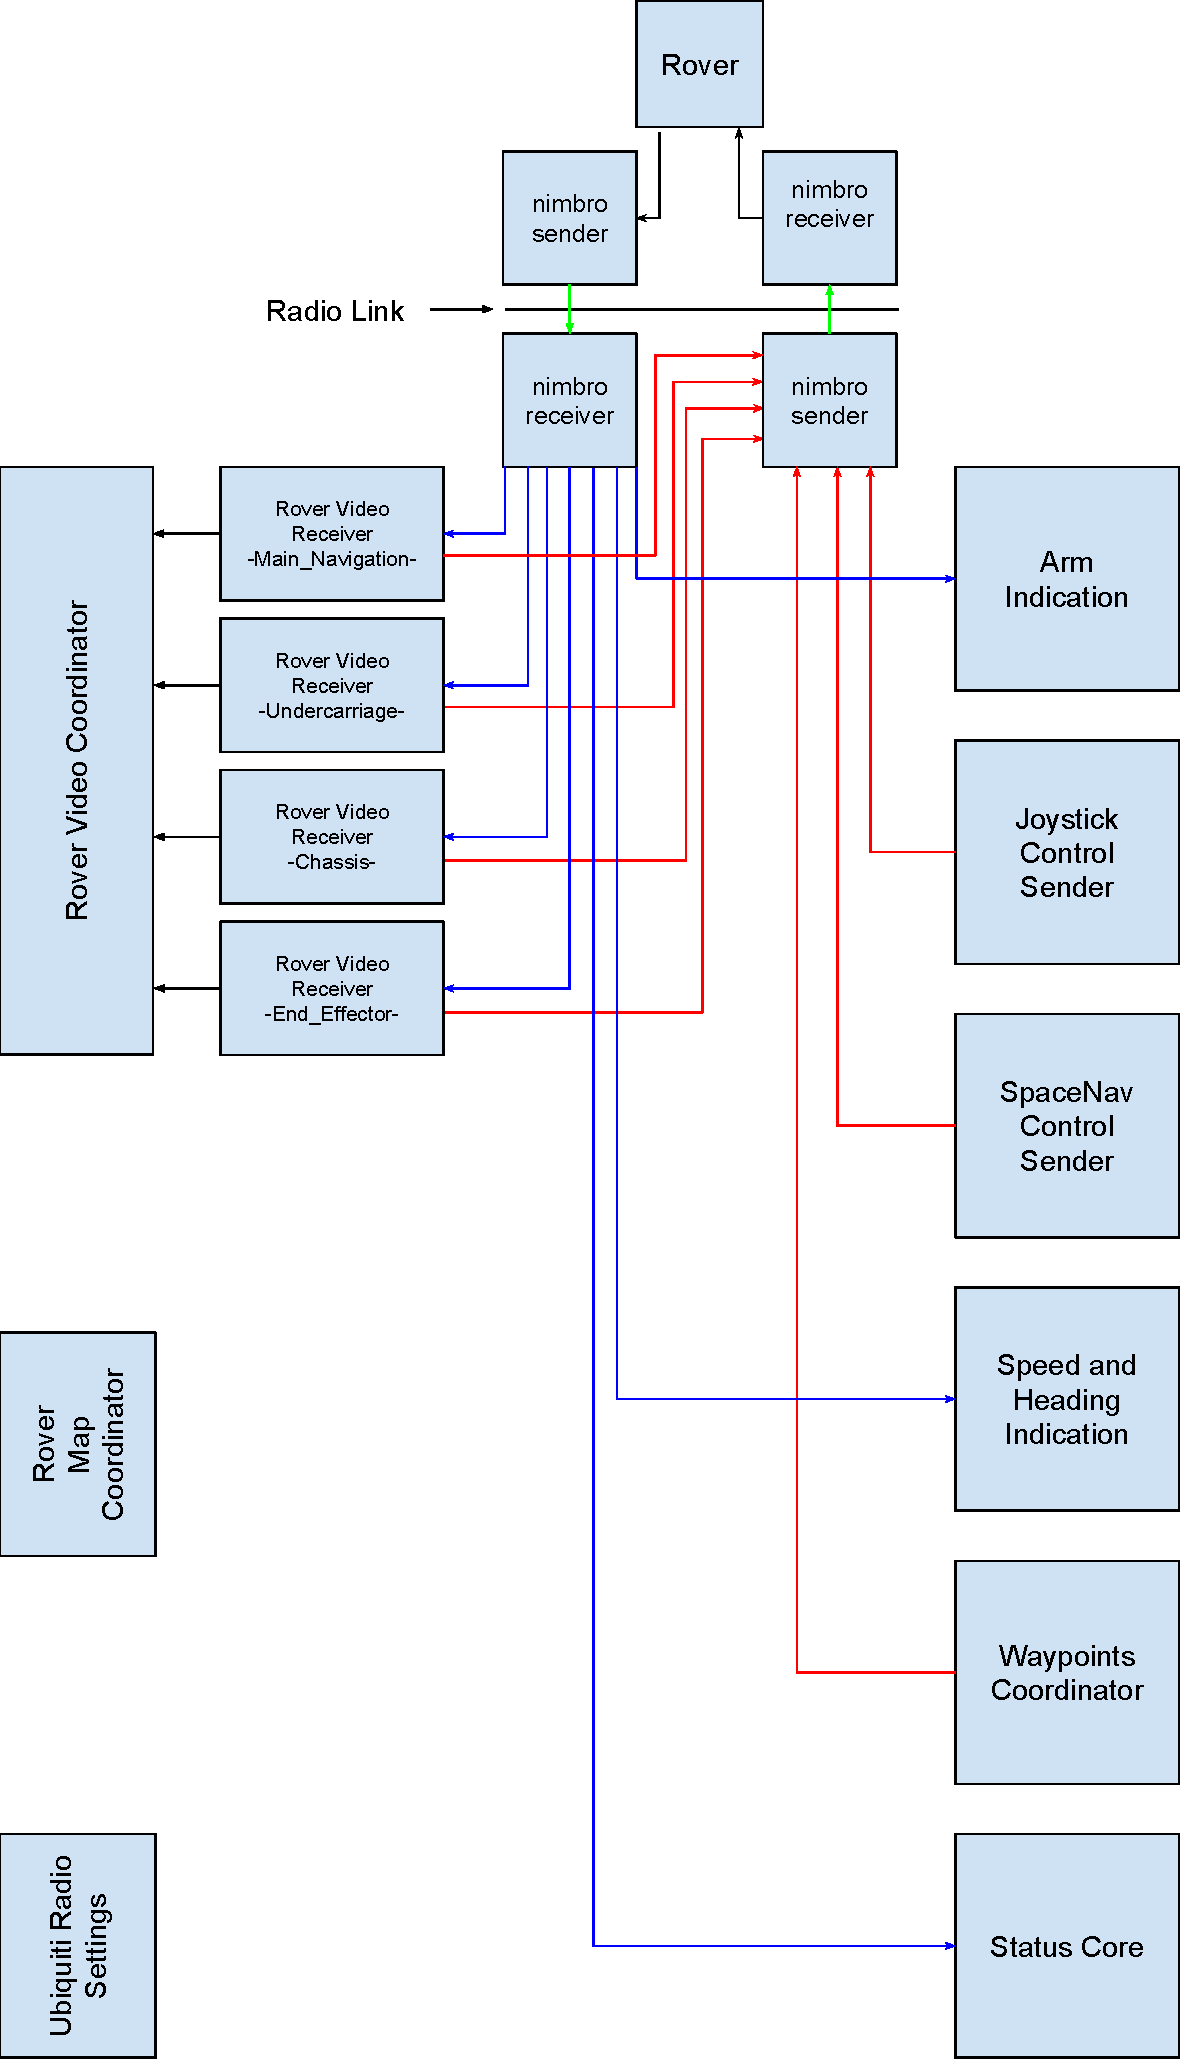
\includepdf[pages=-, scale=0.98]{07-documentation/Rover_Ground_Station_Block_Diagram.pdf}


\subsection{System Requirements}
\subsubsection{Hardware}
\begin{itemize}
\item 1x Computer running Ubuntu 16.04 LTS
	\begin{itemize}
	\item Intel core i5 or i7 equivalent processor
    \item 4GB+ Ram
    \item Minimum two display outputs
	\end{itemize}
\item 2x 1080p Monitors
\item 1x USB Joystick
\item 1x SpaceNav Mouse
\item 1x USB Keyboard
\item 1x USB Mouse
\end{itemize}

\subsubsection{Software / OS}
\begin{itemize}
\item \href{http://wiki.ros.org/kinetic/Installation}{ROS Kinetic}
\item \href{https://www.python.org/}{Python 2.X} with the following packages:
	\begin{itemize}
	\item PyQt5
    \item qdarkstyle
    \item inputs
    \item spnav
    \item Pillow
    \item paramiko
    \item OpenCV 2
    \item qimage2ndarray
    \item numpy
	\end{itemize}
\item Set the computer to an IP address of 192.168.1.15
\end{itemize}


\subsection{How to Install}
\begin{enumerate}
\item Create and \href{http://wiki.ros.org/catkin/Tutorials/create_a_workspace}{setup a catkin workspace} at "$\sim$/catkin\_workspace"
\item Add "source /home/[username]/catkin\_workspace/devel/setup.bash" to the end of your ".bashrc" file, replacing "[username]" with your account's username
\item Create the directory "$\sim$/Github" and clone the \href{https://github.com/OSURoboticsClub/Rover_2017_2018}{Rover\_2017\_2018} repository into it
\item Run the setup script at "$\sim$/Github/Rover\_2017\_2018/software/ground\_station\_setup.sh" to have the proper packages symbolically linked into your new catkin environment and for catkin\_make to be run automatically against it
\item If the catkin\_make process at the end of the script completes with no errors, you're ready to launch the ground station
\end{enumerate}


\subsection{How to Run}
\begin{enumerate}
\item Ensure all hardware from the requirements section above is plugged in
\item Ensure there is a network connection between the ground station computer and Rover
\item Open a terminal and run "roslaunch rover\_main ground\_station.launch"
\item The ground station should launch in full screen across both monitors
\item Press "ctrl-q" at any time to quit the application
\end{enumerate}


\subsection{User Guides}
\subsubsection{Client Requested Quickstart Guide}
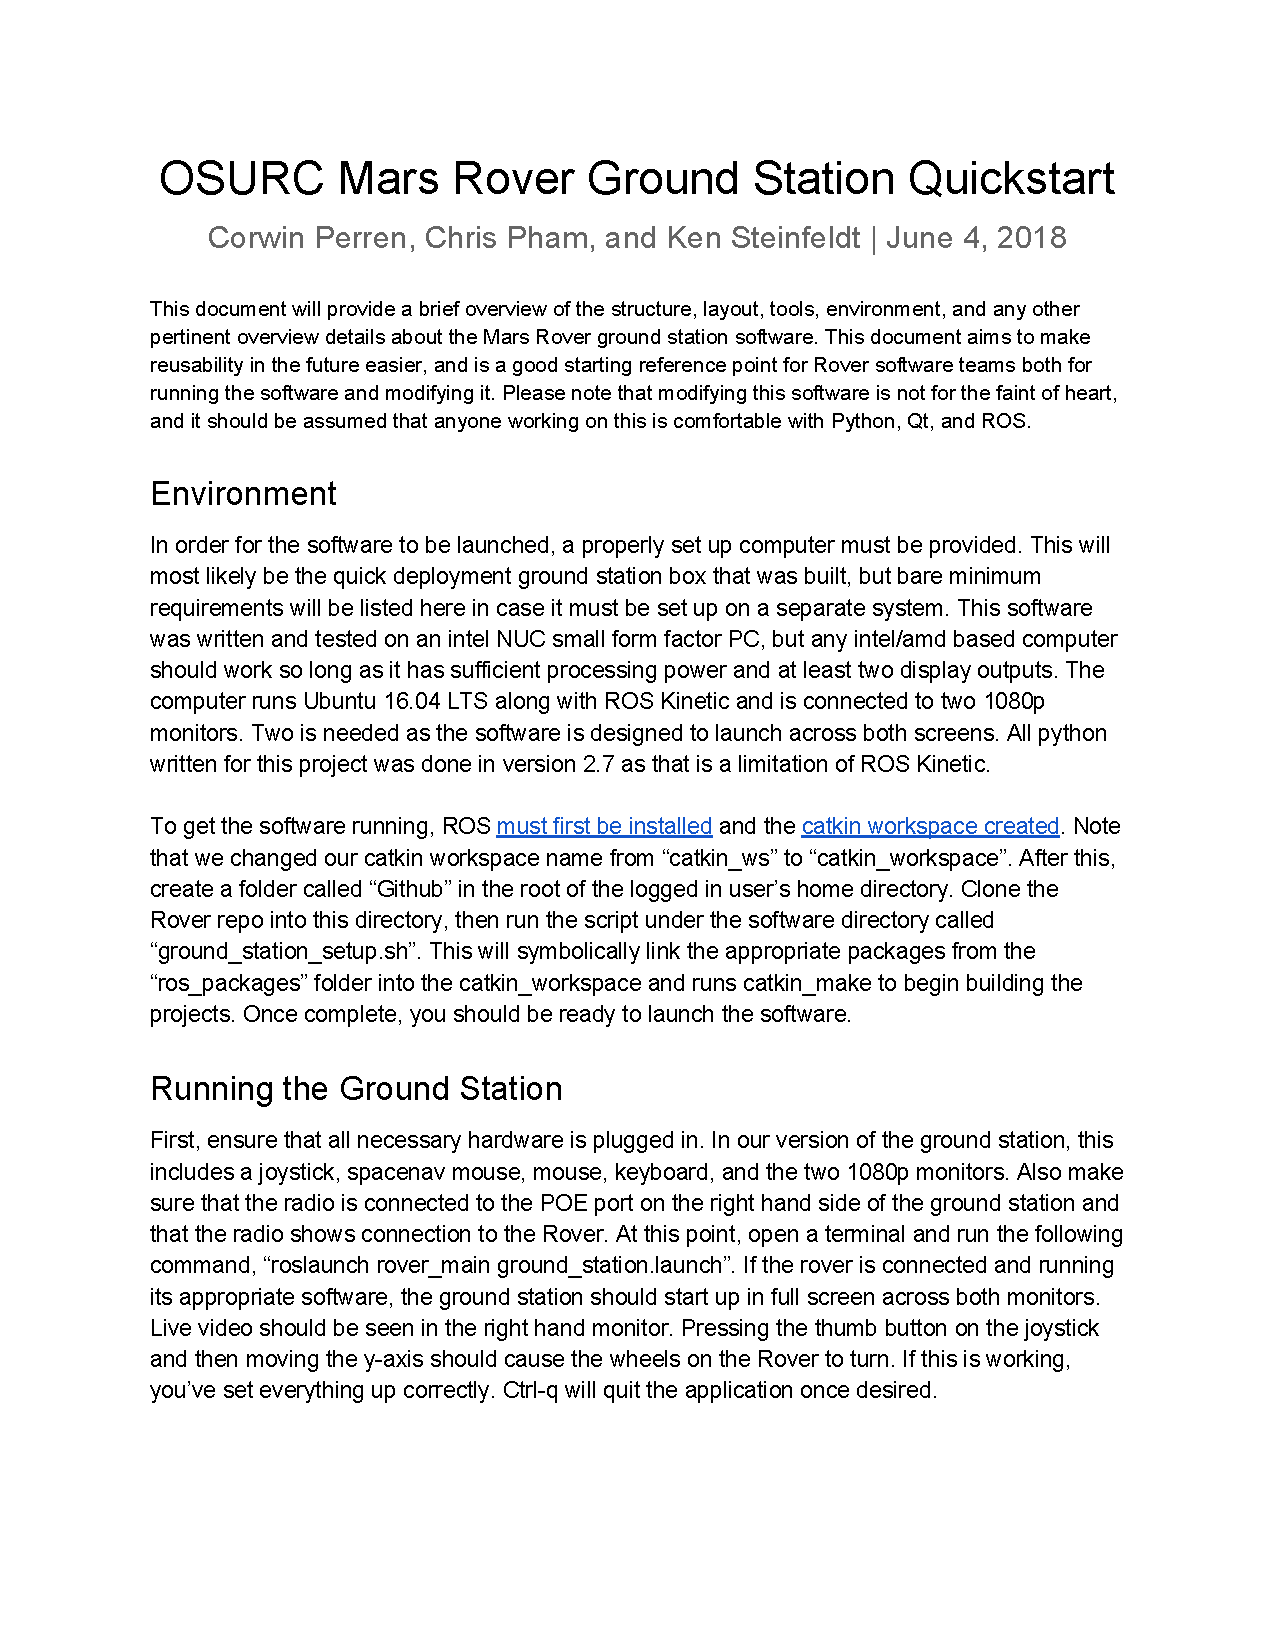
\includepdf[pages=-, frame=true, scale=0.95]{07-documentation/Ground_Station_Quickstart.pdf}
\section{Technical Resources}
\begin{itemize}
\item \href{http://wiki.ros.org/}{ROS Documentation}
\item \href{http://doc.qt.io/}{QT Documentation}
\end{itemize}
\section{Conclusions and Reflections}
\subsection{Chris Pham}
\subsubsection{Week 1}
During the start of the term, I personally did not work on much because of issues with registration 
However, we did work out when we are expecting to work and meet up this term, which would be on Thursdays around 10 o'clock in the morning.
\subsubsection{Week 2}
This week, I worked on completing the integration of the GUI.
It turned out last term, that the East/West portion of the DMS conversion was not being set correctly.
I spent a bit of time trying to get the correct float value to go down but then my minutes was completely off to the calculated DMS of the GPS location.
Turns out that the box that contained the DMS location, would be limited to 0, 90, which actually needs to be 180 because it needs to span a half circle.
Once that value was changed, the values were being set correctly.
\subsubsection{Week 3}
Turns out that I forgot to set the sign of the longitude and latitude to their corresponding North/South and East/West values.
That was easily done using with many possible implementations like equalities, sign function in python, and other things like that.
\subsubsection{Week 4}
This week we worked on fixing our poster and fixing our documentation to fit the new specification that the new competition is now the CIRC (Canadian International Rover Challenge) instead of URC.
\subsubsection{Week 5}
During Week 5, I worked on two important things, multi-threading the downloading of the image files from Google and integration of inputs into my mapping system.

\noindent Multi-threading was done using and starting a list of processes that have access to a download function in the class.
I could not of done a pool because of the issues I was getting like the pickling issues in Python in trying to pack the state.
Another issue that came with this implementation, was the rate limitations that the server was sending.
To combat both issues, I implemented a bounded semaphore instead a normal semaphore, because a bounded version of it will return an error whenever the process tries to obtain a lock.
One big issue is still combining the files because that is still done in square time.
One optimization should be splitting work into its smallest parts and then combining them, however, trying to merge all the files correctly ended up being the biggest issue I had.

\noindent Also have started on integrating the GPS data that we are getting and applying that onto the map system that I've created.
One problem is I forget how the data is formatted in the system and I need direct access to view the data that is being sent by the rover to parse correctly.
\subsubsection{Ken Steinfeldt}

\includepdf[pages=-, frame=true, scale=0.95]{04-techreviewdocs/steinfek-tech-report.pdf}
\subsubsection{Corwin Perren}

\includepdf[pages=-, frame=true, scale=0.95]{04-techreviewdocs/tech_review_perrenc.pdf}

\lstset{ %
  backgroundcolor=\color{white},   % choose the background color
  basicstyle=\footnotesize,        % size of fonts used for the code
  breaklines=true,                 % automatic line breaking only at whitespace
  captionpos=b,                    % sets the caption-position to bottom
  commentstyle=\color{gray},       % comment style
  escapeinside={\%*}{*)},          % if you want to add LaTeX within your code
  keywordstyle=\color{blue},       % keyword style
  stringstyle=\color{purple},      % string literal style
}
\section{Appendix 1: Interesting Code Listings}
\subsection{Drive Test}
\subsubsection{Code}
\begin{lstlisting}[language=python]
class DriveTest(QtCore.QThread):
    def __init__(self):
        super(DriveTest, self).__init__()

        self.not_abort = True

        self.message = None
        self.publisher = rospy.Publisher("/cmd_vel", Twist, queue_size=10)

        rospy.init_node("test")

    def run(self):
        while self.not_abort:
            self.message = Twist()

            self.message.linear.x = 1.0
            self.message.angular.z = 1.0

            self.publisher.publish(self.message)

            self.msleep(100)
\end{lstlisting}

\subsubsection{Description}
This QThread example class starts a ROS publishing node on the "/cmd\_vel" topic to send raw drive control commands to the Rover.
In this case, it is sending a command to drive the Rover forward and to the right, essentially causing it to drive in a never-ending circle.

\subsection{Video Test}
\subsubsection{Code}
\begin{lstlisting}[language=python]
class VideoTest(QtCore.QThread):
    image_ready_signal = QtCore.pyqtSignal()

    def __init__(self, screen_label, video_size=None, sub_path=None):
        super(VideoTest, self).__init__()

        self.not_abort = True

        self.screen_label = screen_label
        self.video_size = video_size

        self.message = None
        self.publisher = rospy.Subscriber(sub_path, CompressedImage, self.__receive_message)

        self.raw_image = None
        self.cv_image = None
        self.pixmap = None
        self.bridge = CvBridge()

        self.image_ready_signal.connect(self.__on_image_update_ready)

    def run(self):
        while self.not_abort:
            if self.raw_image:
                self.cv_image = self.bridge.compressed_imgmsg_to_cv2(self.raw_image, "rgb8")

                if self.video_size:
                    self.cv_image = cv2.resize(self.cv_image, self.video_size)
                    
                self.pixmap = QtGui.QPixmap.fromImage(qimage2ndarray.array2qimage(self.cv_image))
                self.image_ready_signal.emit()
            self.msleep(20)

    def __on_image_update_ready(self):
        self.screen_label.setPixmap(self.pixmap)

    def __receive_message(self, message):
        self.raw_image = message
\end{lstlisting}
\subsubsection{Description}
This example subscribes to the ROS topic that is passed in under the sub\_path argument in order to get video stream data.
An example of this topic might be "/cam1/usb\_cam1/image\_raw/compressed".
Inside of the body of the thread, it checks if there is image data, and if so decompresses it into a raw 8-bit image using ROS's OpenCV bridge libraries.
Finally, it converts the OpenCV image into a QImage and then into a QPixmap before broadcasting an update signal so the main GUI thread can show the image on the QLabel.
It is important to note that any direct GUI updates must happen in the main GUI thread, otherwise the QApplication will crash.

\subsection{Joystick ROS Drive Test}
\subsubsection{Code}
\begin{lstlisting}[language=python]
rospy.init_node("drive_tester")
self.pub = rospy.Publisher("/drive/motoroneandtwo", RoverMotorDrive, queue_size=1)

def __get_controller_data(self):
        if (self.controller_aquired):
            events = self.gamepad.read()

            for event in events:
                if event.code in self.raw_mapping_to_class_mapping:
                    self.controller_states[self.raw_mapping_to_class_mapping[event.code]] = event.state
                    # print "Logitech: %s" % self.controller_states


def __broadcast_if_ready(self):
	drive = RoverMotorDrive()

	axis = self.controller_states["left_stick_y_axis"]

	drive.first_motor_direction = 1 if axis <= 512 else 0
	drive.first_motor_speed = min(abs(self.controller_states["left_stick_y_axis"] - 512) * 128, 65535)

	self.pub.publish(drive)
\end{lstlisting}

\subsubsection{Description}
These two methods and supporting lines above, taken from the testing class LogitechJoystick, contained in the file joystick\_drive\_test.py are the core of what is needed to get joystick data and broadcast it to the rover over a ROS topic.
These two methods are called on after another in a QThread. \_\_get\_controller\_data() reacts to motion events from the joystick and stores the current value of all axes and buttons in self.controller\_states. Then, in \_\_broadcast\_if\_ready(), and instantiation of the custom ROS message type, RoverMotorDrive, is made and values set to a scaled version of the raw values provided by the joystick. Finally, this data is published to the motor drive node and causes the ROS receiving node to see the data, send a message to the motor driver, and cause the motor to spin.

\subsection{Video Test}
\subsubsection{Code}
\begin{lstlisting}[language=python]
def toggle_video_display(self):
	if self.video_enabled:
		if self.video_subscriber:
			self.video_subscriber.unregister()
		self.new_frame = True
		self.video_enabled = False
	else:
		new_topic = self.camera_topics[self.current_camera_settings["resolution"]]
		self.video_subscriber = rospy.Subscriber(new_topic, CompressedImage, self.__image_data_received_callback)
		self.video_enabled = True
\end{lstlisting}
\subsubsection{Description}
This very simple snippet is in the VideoReceiver class in VideoSystems. It is a demonstration of what is needed to properly disable the receiving of video data on a stream. Looking at the Subscriber line, you can see that there is an image callback associated with the subscription to a topic in ROS. This means that if you don't actually unsubscribe (or in this case, unregister) from a topic, as can be seen a few lines above, the data will continue being received even if you are not actively using it. Not doing this would cause unwanted bandwidth to be used.

\subsection{Ubiquiti Channel Change}
\subsubsection{Code}
\begin{lstlisting}[language=python]
GET_CURRENT_CHANNEL_COMMAND = "iwlist ath0 channel"
SET_CHANNEL_COMMAND = "iwconfig ath0 channel"

def setup_and_connect_ssh_client(self):
    self.ssh_client = paramiko.SSHClient()
    self.ssh_client.set_missing_host_key_policy(paramiko.AutoAddPolicy())
    self.ssh_client.connect(ACCESS_POINT_IP, username=ACCESS_POINT_USER, password=ACCESS_POINT_PASSWORD,
                            compress=True)

def apply_channel_if_needed(self):
    if self.channel_change_needed:
        self.show_channel__signal.emit(0)
        self.set_gui_elements_enabled__signal.emit(False)
        self.ssh_client.exec_command(SET_CHANNEL_COMMAND + " %02d" % self.new_channel)
        self.get_and_show_current_channel()
        self.channel_change_needed = False

def get_and_show_current_channel(self):
    channel = 0

    ssh_stdin, ssh_stdout, ssh_stderr = self.ssh_client.exec_command(GET_CURRENT_CHANNEL_COMMAND)
    output = ssh_stdout.read()

    for line in output.split("\n"):
        if "Current Frequency:" in line:
            channel = line.strip("()").split("Channel ")[1]
            break

    self.msleep(500)  # From the gui, this helps show something is actually happening

    self.show_channel__signal.emit(int(channel))
    self.set_gui_elements_enabled__signal.emit(True)
\end{lstlisting}
\subsubsection{Description}
This code shows how we change the 2.4GHz radio channel on the Rocket M2 radios. In the first method, the class initializes an ssh connection to the access point radio. Then, in the thread's main loop, apply\_channel\_if\_needed runs on a regular basis waiting for a channel change to happen. Once it does, it executes an ssh command to change the channel via command line before running a second command via the third method to get the new channel from the radio, parse it, and show it in the GUI. This ensures that if the channel does not get set, the value shown in the GUI will alert the user to this fact.

\subsection{Compass Rotation}
\subsubsection{Code}
\begin{lstlisting}[language=python]
ROTATION_SPEED_MODIFIER = 2.5

def rotate_compass_if_needed(self):
    heading_difference = abs(int(self.shown_heading) - self.current_heading)
    should_update = False

    if heading_difference > ROTATION_SPEED_MODIFIER:
        self.shown_heading += self.rotation_direction * ROTATION_SPEED_MODIFIER
        self.shown_heading %= 360
        should_update = True
    elif heading_difference != 0:
        self.shown_heading = self.current_heading
        should_update = True

    if should_update:
        self.current_heading_shown_rotation_angle = int(self.shown_heading)

        if self.current_heading_shown_rotation_angle != self.last_current_heading_shown:
            new_compass_image = self.main_compass_image.rotate(self.current_heading_shown_rotation_angle, resample=PIL.Image.BICUBIC)
            self.last_current_heading_shown = self.current_heading_shown_rotation_angle

            self.compass_pixmap = QtGui.QPixmap.fromImage(ImageQt(new_compass_image))
            self.show_compass_image__signal.emit()

def update_heading_movement(self):
    current_minus_shown = (self.current_heading - self.shown_heading) % 360

    if current_minus_shown >= 180:
        self.rotation_direction = -1
    else:
        self.rotation_direction = 1
\end{lstlisting}
\subsubsection{Description}
This code shows how movement updates to the compass are made. The second method gets called when a new heading change is made, setting whichever rotation direction is shorter to reach the desired goal. Then, in the main loop, the upper method calculates the difference between the current shown heading and the actual heading determining whether it should be moving or not. If it should, the main compass image that was loaded during init is rotated via a bicubic sampling algorithm to maintain image clarity, converted to a QPixmap, before an update signal is broadcast to the main thread to show the image.
\section{Appendix 2}
\subsection{Ground Station Final Photos}
\begin{figure}[h!]
  \centering
  \captionsetup{justification=centering}
  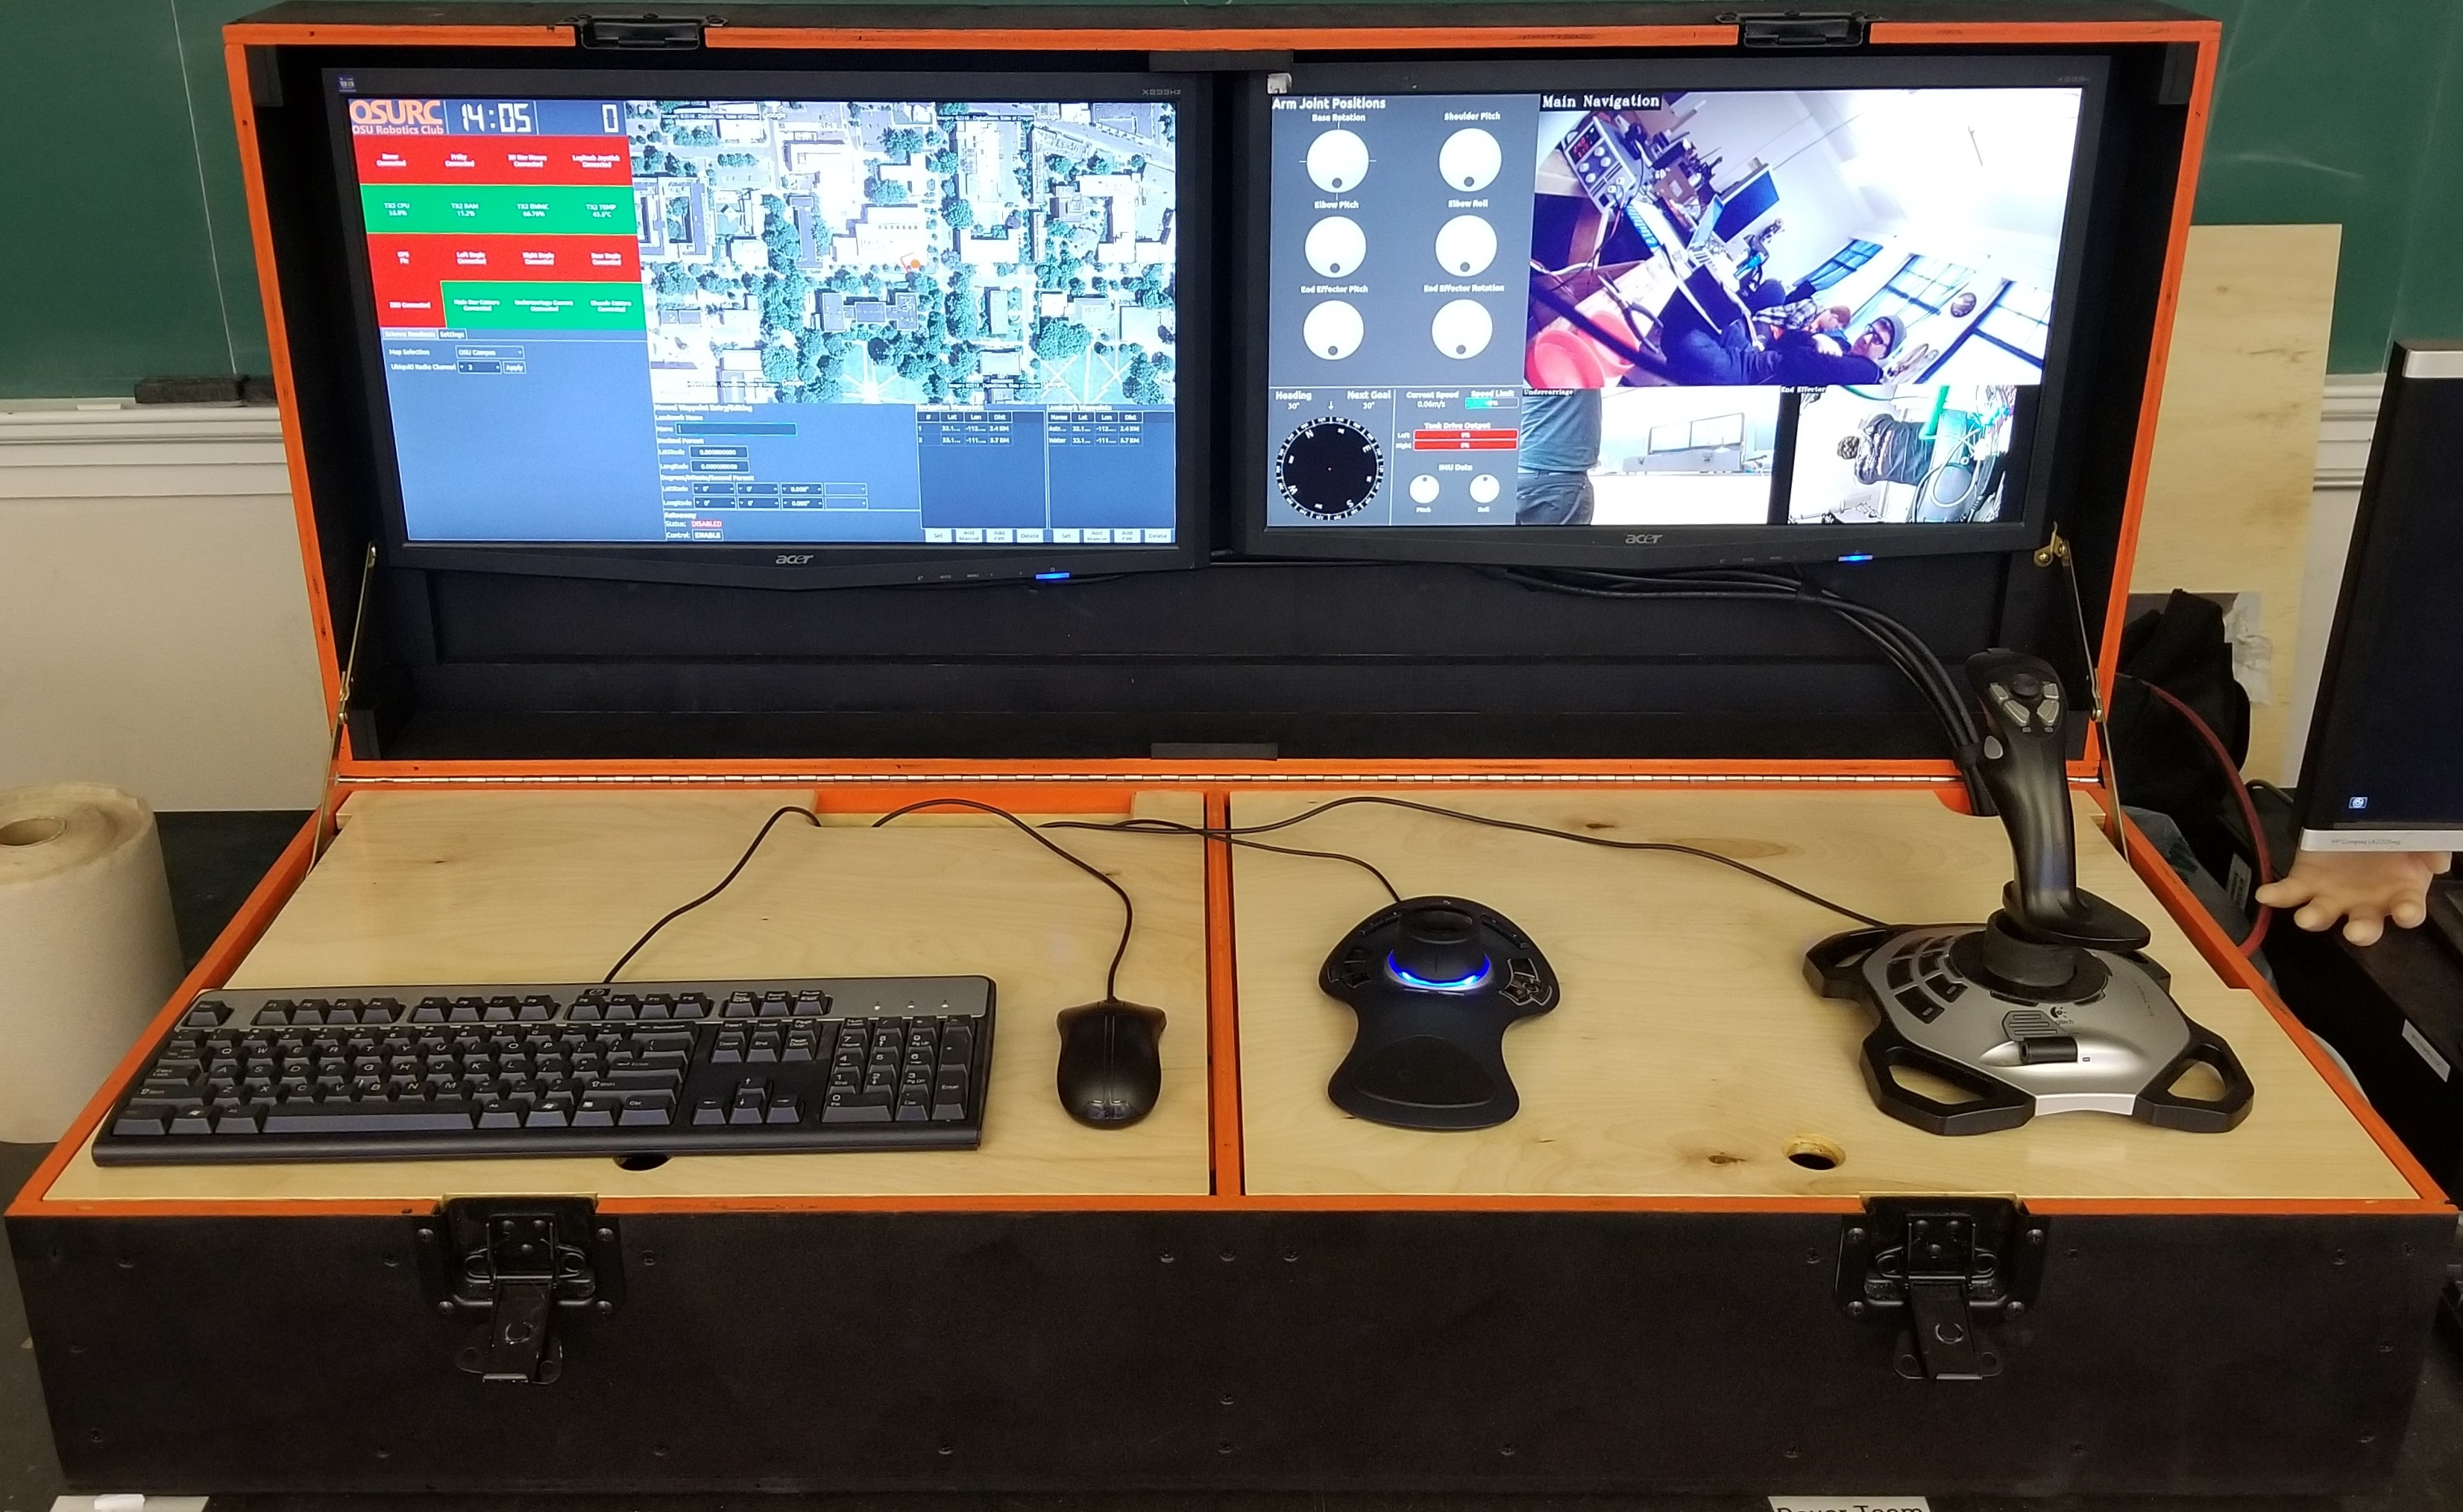
\includegraphics[width=0.9\textwidth]{misc_media/ground_station_framed}
  \caption{Finished Ground Station Hardware}
\end{figure}

\begin{figure}[h!]
  \centering
  \captionsetup{justification=centering}
  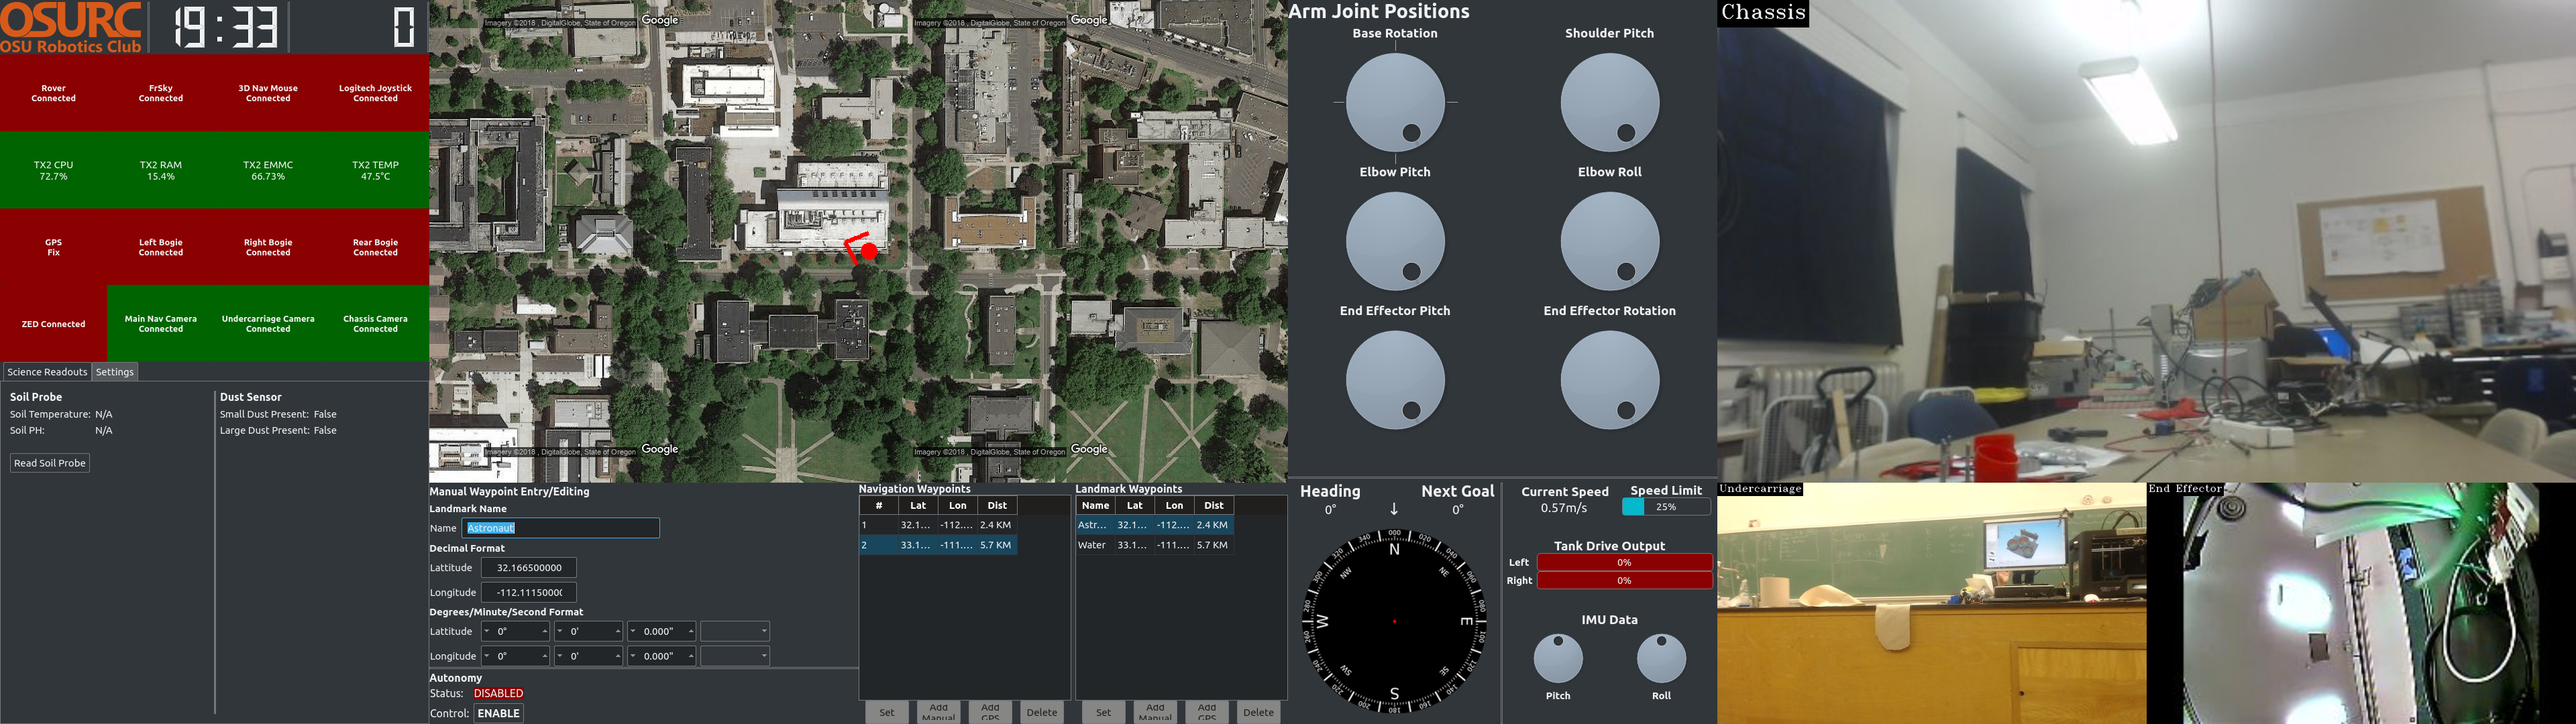
\includegraphics[width=0.9\textwidth]{misc_media/ground_station_screenshot}
  \caption{Finished Ground Station Screenshot}
\end{figure}

\begin{figure}[h!]
  \centering
  \captionsetup{justification=centering}
  \includegraphics[width=0.9\textwidth]{misc_media/ground_station_expo}
  \caption{Finished Ground Station at Expo}
\end{figure}

\begin{figure}[h!]
  \centering
  \captionsetup{justification=centering}
  \includegraphics[width=0.9\textwidth]{misc_media/ground_station_expo_2}
  \caption{Chatting with TA at Expo}
\end{figure}
\end{document}





